%iffalse
\let\negmedspace\undefined
\let\negthickspace\undefined
\documentclass[journal,12pt,onecolumn]{exam}
\usepackage[version=4]{mhchem}
\usepackage{chemformula} % for \ch if needed
\usepackage{chemfig}
\usepackage{chemmacros}
\chemsetup{modules = reactions} % Enables reaction arrows
\usepackage{graphicx}
\graphicspath{ {./images/} }
\usepackage{geometry}
\usepackage{lastpage}
\usepackage{cite}
\usepackage{amsmath,amssymb,amsfonts,amsthm}
\usepackage{enumitem,multicol}
\usepackage{algorithmic}
\usepackage{graphicx}
\usepackage{textcomp}
\usepackage{xcolor}
\usepackage{txfonts}
\usepackage{listings}
\usepackage{enumitem}
\usepackage{mathtools}
\usepackage{gensymb}
\usepackage{comment}
\usepackage[breaklinks=true]{hyperref}
\usepackage{tkz-euclide} 
\usepackage{listings}
\usepackage{gvv}                                        
%\def\inputGnumericTable{}                                 
\usepackage[latin1]{inputenc}                                
\usepackage{color}                                            
\usepackage{array}                                            
\usepackage{longtable}                                       
\usepackage{calc}                                             
\usepackage{multirow}                                         
\usepackage{hhline}                                           
\usepackage{ifthen}                                           
\usepackage{lscape}
\usepackage{tabularx}
\usepackage{array}
\usepackage{float}


\newtheorem{theorem}{Theorem}[section]
\newtheorem{problem}{Problem}
\newtheorem{proposition}{Proposition}[section]
\newtheorem{lemma}{Lemma}[section]
\newtheorem{corollary}[theorem]{Corollary}
\newtheorem{example}{Example}[section]
\newtheorem{definition}[problem]{Definition}
\newcommand{\BEQA}{\begin{eqnarray}}
\newcommand{\EEQA}{\end{eqnarray}}
\newcommand{\define}{\stackrel{\triangle}{=}}
\theoremstyle{remark}

\geometry{margin=1 in}



\setlength{\headheight}{14pt}
\setlength{\headsep}{5pt}
\setlength{\footskip}{20pt}

\begin{document}
\begin{enumerate}
    

 \section{Q.1-Q.25 carry one mark each.}

\item 
    The critical speed (revolutions per unit time) of a ball mill of radius R, which uses balls of radius r, is 
\hfill{(GATE 2010 CH)}\\

\begin{figure}[htbp]
    \centering
    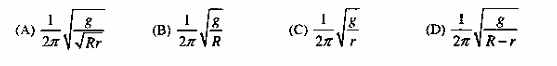
\includegraphics[width=1\columnwidth]{figs/Q.1 options.png}
    \caption{options}
    \label{fig:figs/Q.1 options.png}
\end{figure}
  

\item 
   The ratio of Nusselt number to Biot number is
   \hfill{(GATE 2010 CH)}\\
\begin{enumerate}
    \item conductive resistance of fluid / conductive resistance of solid
    \item conductive resistance of fluid / convective resistance of fluid
    \item conductive resistance of solid / conductive resistance of fluid 
    \item unity
\end{enumerate}
\item
  The ratio of thermal boundary layer thickness to the concentration boundary layer thickness is proportional to
  
  \hfill{(GATE 2010 CH)}\\
  
\begin{enumerate}
  \item Nu
  \item Le
  \item Sh
  \item Pr
\end{enumerate}
 \item 
  For a first order isothermal catalytic reaction, A $--->$ P, occuring in an infinitely long cylindrical pore, the relationship between effectiveness factor,
  
\hfill{(GATE 2010 CH)}

\begin{figure}[htbp]
    \centering
    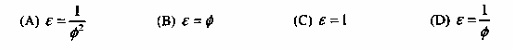
\includegraphics[width=1\columnwidth]{figs/Q.4 optons.png}
    \caption{options}
    \label{fig:figs/Q.4 optons.png}
\end{figure}
     
\item
  Match the location of the poles/zeros in the s-plane, listed in GROUP I, with the system response characteristics in GROUP II.
  
\hfill{(GATE 2010 CH)}\\

 \begin{center}
\begin{tabular}{ll}
    \textbf{Group I} & \textbf{Group II} \\
    P. Ferrite & 1. Hexagonal Close Packed (HCP) \\
    Q. Austenite & 2. Body Centered Cubic (BCC) \\
    R. Martensite & 3. Body Centered Tetragonal (BCT) \\
    & 4. Face Centered Cubic (FCC)
\end{tabular}
\end{center}
    
  
\begin{enumerate}
    \item P-I,Q-II,R-III
    \item P-III,Q-IV,R-I
    \item P-III,Q-II,R-IV
    \item P-I,Q-IV,R-III
    
\end{enumerate}
         
    \item 
    Which ONE of the following statements about baffles in a shell and tube heat exchanger is FALSE? Baffles
   
\hfill{(GATE 2010 CH)}\\
   
    \begin{enumerate}
    
        \item act as a support to the tube bundle
        \item reduce the pressure drop on the shell- side
        \item alter the shell-side flow pattern
        \item help in increasing the shell-side heat transfer coefficient
    \end{enumerate}
\item 
    The term, Knuckle radius, is associated with
   
   \hfill{(GATE 2010 CH)}\\
   
   \begin{enumerate}
       \item flat heads
       \item torispherical heads
       \item hemispherical heads
       \item conical heads
   \end{enumerate}
   
  \item 
   Inthe manufacture of caustic soda from brine, which ONE of the following statements is TRUE?
   
  \hfill{(GATE 2010 CH)}\\
   
   \begin{enumerate}
       \item The membrane cell CANNOT produce concentrated NaOH solution, and CANNOT tolerate calcium and magnesium ions in the feed brine.
       \item The membrane cell CANNOT produce concentrated NaOH solution, CAN tolerate calcium and magnesium ions in the feed brine
       \item  The membrane cell CAN produce concentrated NaOH solution, CANNOT tolerate calcium and magnesium ions in the feed brine 
       \item  The membrane cell CAN produce concentrated NaOH solution, CAN tolerate calcium and magnesium ions in the feed brine
   \end{enumerate}

   \item 
   For making superphosphate by acidulation of phosphate rock, use of nitric acid is desirable, because
   
\hfill{(GATE 2010 CH)}\\

   \begin{enumerate}
       \item nitric acid is less expensive than sulphuric acid
       \item the availability of nitrogenenhances the value of the superphosphate as a fertiliser
       \item the process produces non-hygroscopic superphosphate
       \item the process produces superphosohate having higher phosphorous content than the sulphuric acid process
   \end{enumerate}


 \item 
   Match the process in GROUP I with the process in GROUP II.

\hfill{(GATE 2010 CH)}\\
  
      \begin{tabular}{|c|c|c|}
     \hline
     \textbf{Mineral} & \textbf{Modal abundance \brak{\%}} & \textbf{Partition coefficient}\\
     \hline
     Clinopyroxene & $45$ & $0.506$ \\
      \hline
      Orthopyroxene & $40$ & $0.42$ \\
      \hline
      Olivine & $10$ & $0.045$ \\
      \hline
      Plagioclase & $05$ & $0.019$ \\
      \hline
\end{tabular}

    \begin{enumerate}
        \item P-I,Q-II,R-III
        \item P-II,Q-I,R-III
        \item P-III,Q-I,R-II
        \item P-III,Q-II,R-I
    \end{enumerate}
\item 
 The inverse of the matrix \[
 \begin{bmatrix}
     1 & 2\\
     3 & 4
 \end{bmatrix}  is
 \] 
 
\hfill{(GATE 2010 CH)}\\

\begin{figure}[H]
    \centering
    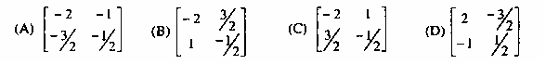
\includegraphics[width=1\columnwidth]{figs/q.11 OPTIONS.png}
    \caption{options}
    \label{fig:figs/q.11 OPTIONS.png}
\end{figure}
\item 
  The Laplace transform of the function shown in the figure below is
 \hfill{(GATE 2010 CH)}\\

\begin{figure}[H]
    \centering
    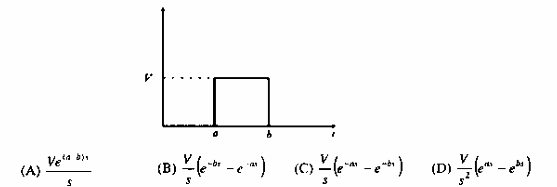
\includegraphics[width=1\linewidth]{figs/q.12 image.png}
    \caption{options}
    \label{fig:figs/q.12 image.png}
\end{figure}
\item 
 The Maxwell-Boltzmann velocity distribution for the x- component of the velocity, at temparature T, is 
 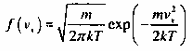
\includegraphics[width=0.25\linewidth]{figs/Q.13 image.png}. The standard deviation of the distribution is
 
\hfill{(GATE 2010 CH)}\\
    
    \begin{figure}[H]
        \centering
        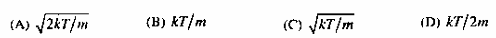
\includegraphics[width=01\linewidth]{figs/Q.13 options.png}
        \caption{options}
        \label{fig:figs/Q.13 options.png}
    \end{figure}
 \item 
 Given that $i=\sqrt{-1}$, $i^i$ is equal  to
     
    \hfill{(GATE 2010 CH)}\\

  \begin{figure}[H]
      \centering
      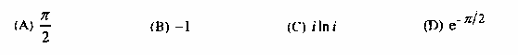
\includegraphics[width=1.0\linewidth]{figs/Q.14 options.png}
      \caption{options}
      \label{fig:figs/Q.14 options.png}
  \end{figure}
\item 
 A root of the equation $x^4$ - 3x +1=0 needs to be found using the Newton-Raphson method. If the initial guess, x is taken as 0, then the new estimate ,x1 after the first iteration is 
 
 \hfill{(GATE 2010 CH)}\\
 
\begin{enumerate}
    \item 1/3
    \item -1/3
    \item 3
    \item -3
 \end{enumerate}
\item 
   An equimolar liquid mixture of species 1 and 2 is in equilibrium with its vapour at 400K. At this temparature, the vapour pressure of the species are P1 = 180 kPa and P2 =120kPa. Assuming that Raoult's law is valid, the value of y1 is
 
 \hfill{(GATE 2010 CH)}\\

 \begin{enumerate}
     \item 0.30
     \item 0.41
     \item 0.50
     \item 0.60
 \end{enumerate}
\item 
 A new linear temparature scale, denoted by 'S, has been developed, where the freezing point of water is 200'S and boiling point of water is 400'S. On this scale, 500'S corresponds, in degree celsius, to
 \hfill{(GATE 2010 CH)}\\

 \begin{enumerate}
     \item 100'C
     \item 125'C
     \item 150'C
     \item 300'C

 \end{enumerate}
\item 
  A saturated liquid at 1500 kPa and 500 K,with an enthalpy of 750 kJ/kg,is throttled to a liquid-vapour mixture at 150 kPa and 300K .At the exit conditions, the enthalpy of the saturated liquid is 500 kJ/kg and the enthalpy of the saturated vapour is 2500 kJ/kg.The percentage of the original liquid, which vapourizes, is
 \hfill{(GATE 2010 CH)}\\

 \begin{enumerate}
     \item 87.5%
     \item 67%
     \item 12.5%
     \item 10%
     
 \end{enumerate}
\item 
   The stream function in a xy- plane is given below:
 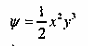
\includegraphics[width=0.125\linewidth]{figs/Q.19 image.png}

   The velocity vector for this stream function is

   \hfill{(GATE 2010 CH)}\\

  \begin{figure}[H]
      \centering
      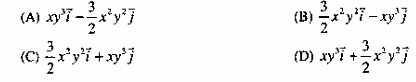
\includegraphics[width=1.0\linewidth]{figs/Q.19 options.png}
      \caption{options}
      \label{fig:figs/Q.19 options.png}
  \end{figure}
\item 
   The height of a fluidized bed at incipient fluidization is 0.075 m, and the corresponding voidage is 0.38. If the voidage of the bed increases to 0.5, then the height of the bed would be
\hfill{(GATE 2010 CH)}\\

\begin{enumerate}
    \item 0.058m
    \item 0.061m
    \item 0.075m
    \item 0.093m
\end{enumerate}
\item
   A storage vessel exposed to atmosphere (absolute pressure = 10.3 m of water ) has a diameter of 3m and is initially filled with water to a hieght of 2m. The pump draws water from the vessel and is located at an elevation of 5m above the bottom of the vessel. The frictional head loss in the suction pipe is 2m of water. If the vapour pressure of the liquid at the temparature of operation is 3m of water. then the available NPSH is

   \hfill{(GATE 2010 CH)}\\

 \begin{figure}[H]
     \centering
     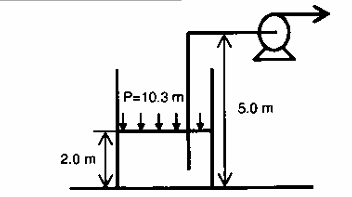
\includegraphics[width=0.5\linewidth]{figs/Q.21 image.png}
     \caption{options}
     \label{fig:figs/Q.21 image.png}
 \end{figure}
 
  \begin{enumerate}
      \item 2.3m
      \item 5.3m
      \item 6.3m
      \item 8.3m
      
  \end{enumerate}
\item
 In Hagen-Poiseuille flow through a cylindrical tube, the radial profile of shear stress is
 
 \hfill{(GATE 2010 CH)}\\

\begin{enumerate}
    \item constat
    \item cubic
    \item parabolic
    \item linear
    
\end{enumerate}
\item 
  Flow measuringinstruments with different specifications (zero and span) are available for an application that requires flow rate measurementsin the range of 300 litres/h to 400 litres/h. The appropriate instrument for this application is the ONE whose specifications are
  \hfill{(GATE 2010 CH)}\\

  \begin{enumerate}
      \item zero = 175litres/h,span = 150litres/h
      \item zero = 375litres/h, span = 100litres/h
      \item zero = 275litres/h, span = 150litres/h
      \item zero = 475litres/h, span = 100litres/h
  \end{enumerate}
\item 
   The transfer function, G(s), whose asymptote Bode diagram is shown below, is\\

\begin{figure}[H]
    \centering
    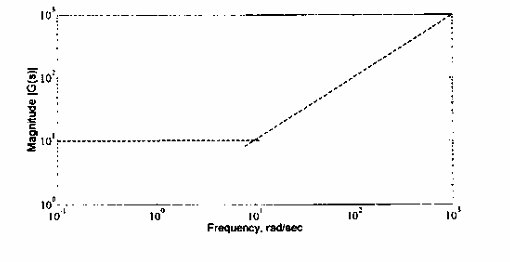
\includegraphics[width=1\linewidth]{figs/Q.24 image.png}
    \caption{options}
    \label{fig:figs/Q.24 image.png}
\end{figure}
      
    
 \hfill{(GATE 2010 CH)}\\


   \begin{enumerate}
       \item 10s+1
       \item s-10
       \item s+10
       \item 10s-1
   \end{enumerate}
\item 
   The flooding velocity in a plane coloumn, operating at 1 atm pressure, is 3 m/s. If the coloumn is operated at 2 atm pressure, under otherwise identical comditions, the flooding velocity will be
   
\hfill{(GATE 2010 CH)}\\

 \begin{enumerate}
   
  \item  3/$\sqrt{2}$\\
  \item  3/2\\
  \item  1\\
  \item  3/4\\   
\end{enumerate}

 
  
  \section{Q.26-Q.55 carry two mark each.}
\item 
   The solution of the differential equation
   \begin{equation}
       d^2y/dt^2 + 2dy/dt + 2y = 0
   \end{equation}
   with the initial conditions y(0) = 0, (dy/dt) at t=0 = -1, is
\hfill{(GATE 2010 CH)}\\

\begin{enumerate}
    \item -tsint
    \item -$e^-t$(1-cost)\\
    \item -(t+sint)/2
    \item -$e^-t$ sint
\end{enumerate}
\item 
 If u = y i + xy j and v = $x^2$ j, then curl(u X v) is

 \hfill{(GATE 2010 CH)}\\
 
 \begin{enumerate}
     \item (2x$y^3$)i - (x+ $y^2$)j
     \item (xy-$x^2$)i - (y-3xy)j
     \item (2$x^2y^2$-3$x^3$)i - ($y^3$-3x$y^2$)k
     \item (3x$y^2$-$x^3$)i - ($y^3-3x^2$y)j
 \end{enumerate}
\item 
 X and Y are independent random variables, X follows a binomial distribution, with N = 5 and p = 1/2 .Y takes integer values 1 and 2, with equal probability. Then the probability that X=Y is
 \hfill{(GATE 2010 CH)}\\

 \begin{enumerate}
     \item 15/64
     \item 15/32
     \item 1/2
     \item 15/16
     
 \end{enumerate}
\item 
  A box contains three red and two black balls. Four balls are removed from the box one by one ,without replacement. The probability of the ball remaining in the box being red, is

  \hfill{(GATE 2010 CH)}\\

  \begin{enumerate}
      \item 609/625
      \item 3/5
      \item 2/5
      \item 81/625
  \end{enumerate}
 \item 
   For a function g(x), if g(0)=0 and g'(0)=2, then

\begin{figure}[H]
    \centering
    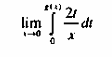
\includegraphics[width=0.25\linewidth]{figs/Q.30 image.png}
    \caption{options}
    \label{fig:figs/Q.30 image.png}
\end{figure}
   
   
    is equal to
\hfill{(GATE 2010 CH)}\\

\begin{enumerate}
    \item $\infty$
    \item 2
    \item 0
    \item -$\infty$
\end{enumerate}
\item 
 At constant T and P, the molar density of a binary mixture is given by P = 1+x`, where x` is the mole fraction of component 2. The partial molar volune at infinite dilution for component 1, V1`, is
 \hfill{(GATE 2010 CH)}\\

 \begin{enumerate}
     \item 0.75
     \item 1.0
     \item 2.0
     \item 4.0
 \end{enumerate}
 \item
 A saturated solution at 30'C contains 5 moles of solute (M.W = 50kg/kmol) per kg of solvent (M.W =20kg/kmol). The solubility at 100'C is 10 moles of the solute per kg of the solvent. If 10kg of the original solution is heated to 100'C, then the weight of the additional solute that can be dissolved in it, is
 \hfill{(GATE 2010 CH)}\\

 \begin{enumerate}
     \item 0.25 kg
     \item 1 kg
     \item 2 kg
     \item 3.34 kg
     
 \end{enumerate}
\item
  The products of combustion of methane in atmosphere air (21\% O2 and  79\% N2) have the following composition on a dry basis:

      \begin{table}[htbp]
  \centering
  \caption{Table-3}
  \label{table3}
  \begin{tabular}{cc}
  \textbf{Processing Technique} & \textbf{Producct} \\ \\
    P. Calendering & 1. Pipes \\
    Q. Extrusion & 2. Disposable cups \\
    R. Injection moulding & 3. Sheets \\
    S. Thermoforming & 4. Nylon gears \\
  \end{tabular}
\end{table}
    The ratio of the moles of CH4 to the moles of O2 in the feed stream is 
  
  \hfill{(GATE 2010 CH)}\\

  \begin{enumerate}
      \item 1.05
      \item 0.60
      \item 0.51
      \item 0.45
  \end{enumerate}
\item 
   A hydrometer, with stem cross-sectional area of 2.82x $10^-5 m^2$. is immersed in a very large vessel containing water as shown in figure.The immersed volume is 15x$10^-6 m^3$ and the length of the stem above water is Lw.If the entire volume of water is replaced by a liquid with specific gravity 1.5 and if the length of the stem above liquid surface is Lf, then the difference , Lf-Lw, is
   
   \hfill{(GATE 2010 CH)}\\
   
\begin{figure}[H]
    \centering
    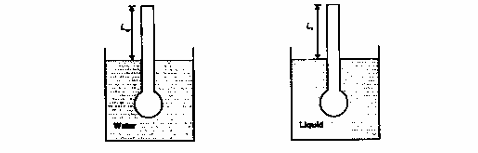
\includegraphics[width=1.0\linewidth]{figs/Q.34 image.png}
    \caption{figure}
    \label{fig:figs/Q.34 image.png}
\end{figure}
     
    \begin{enumerate}
        \item -177 mm
        \item 177 mm
        \item -266 mm
        \item 266 mm
        
    \end{enumerate}
\item 
  The diameter of a drop of a liquid fuel changes with time, due to combustion, according to the relationship, D = D' (1- t/t'). While burning, the drop falls at its terminal velocity under Stoke's flow regime. The distance it will travel before it complete combustion, is given by
 
 \hfill{(GATE 2010 CH)}\\

\begin{figure}[H]
    \centering
    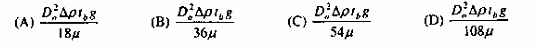
\includegraphics[width=1.0\linewidth]{figs/Q.35 options.png}
    \caption{options}
    \label{fig:figs/Q.35 options.png}
\end{figure}
\item 
 The figure below shows steady state temparature profiles for one dimensional heat transfer within a solid slab for the following cases:

  P: uniform heat generation    with left surface perfectly insulated
  
  Q: uniform heat generation    with right surface perfectly insulated
  
   R: uniform heat consumption    with left surface perfectly insulated
   
   S: uniform heat consumptiom    with right surface perfectly insulated \\

 \begin{figure}[H]
     \centering
     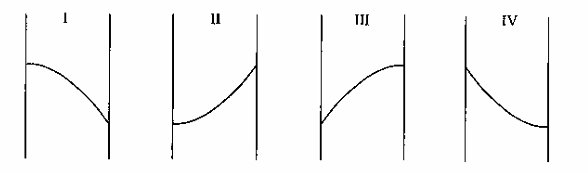
\includegraphics[width=1.0\linewidth]{figs/Q.36 image.png}
     \caption{figure}
     \label{fig:figs/Q.36 image.png}
 \end{figure}
    
    Match the profiles with appropriate cases.
\hfill{(GATE 2010 CH)}\\

   \begin{enumerate}
    \item P-I,Q-III,R-II,S-IV
    \item P-II,Q-III,R-I,S-IV
    \item P-I,Q-IV,R-II,S-III
    \item P-II,Q-IV,R-I,S-III
   \end{enumerate}
\item 
    The view factor matrix for two infinitely long co-axial cylinders, shown in the figurebelow, is

 \begin{figure}[H]
     \centering
     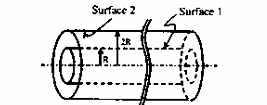
\includegraphics[width=0.5\linewidth]{figs/Q.37 image.png}
     \caption{figure}
     \label{fig:figs/Q.37 image.png}
 \end{figure}
     
\hfill{(GATE 2010 CH)}\\


\begin{enumerate}

    \item $\begin{bmatrix}
       0 & 1\\
        0.5 & 0.5
    \end{bmatrix}$
    \item $\begin{bmatrix}
       0 & 1\\
        1 & 0
    \end{bmatrix}$
    \item $\begin{bmatrix}
        1 & 0\\
        0 & 1
    \end{bmatrix}$
    \item $\begin{bmatrix}
       0.5 & 0.5\\
        0 & 1
    \end{bmatrix}$
\end{enumerate}
\item 
  At 25'C and 90\% relative humidity, water evaporates from the surface of the lake at the rate of 1.0 kg/$m^2$/h. The relative humidity that lead to an evaporation rate of 3.0 kg/$m^2$/h, with other conditions remaining the same, is

\hfill{(GATE 2010 CH)}\\

 \begin{enumerate}
     \item 30\%
     \item 50\%
     \item 60\%
     \item 70\%
 \end{enumerate}
\item 
 A liquid flows over a flat napthalene plate of length L, at a Reynolds number (Re = Lpu'/$\mu$) of 1500, as shown in the figure. The surface concentration of napthalene is $Ca > C\infty$ . and the surface temparature is $Tf > T\infty$. Assume Pr = Sc = 1.

 \hfill{(GATE 2010 CH)}\\

\begin{figure}[H]
    \centering
    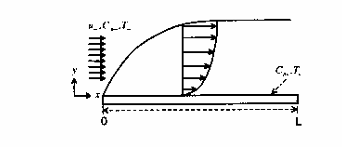
\includegraphics[width=0.5\linewidth]{figs/Q.39 image.png}
    \caption{figure}
    \label{fig:figs/Q.39 image.png}
\end{figure}

   If, at 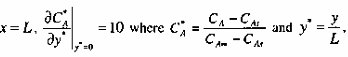
\includegraphics[width=0.5\linewidth]{figs/Q.39 image-2.png} , then the Nusselt number and the friction co-efficient at x = L, are

    \begin{enumerate}
        \item 10,1/75
        \item 10,10
        \item 20,10
        \item 1/75,10
        
    \end{enumerate}
\item 
   Two reactors (reactor 1 and reactor 2) with average residence times, $\tau1$ and $\tau2$. respectively are placed in series. Reactor 1 has zero dispersion and reactor 2 has infinite dispersion. The residence time distribution, E(t) of this system is given by
    \hfill{(GATE 2010 CH)}\\

\begin{figure}[H]
    \centering
    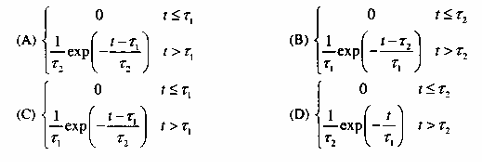
\includegraphics[width=1.0\linewidth]{figs/Q.40 options.png}
    \caption{options}
    \label{fig:figs/Q.37 image.png}
\end{figure}
\item 
 An autocatalytic liquid phase reaction, A + R $\rightarrow$ 2R is conducted in an isolated batch reactor with a small initial concentrationof R. Assume that the order of reaction with respect to both reactants is positive. The rate of reaction (-Ra) versus concentration Ca, as the reaction proceeds, is depicted by 

\hfill{(GATE 2010 CH)}\\
 
 \begin{figure}[H]
     \centering
     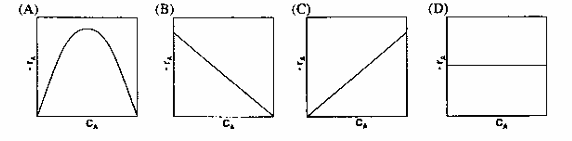
\includegraphics[width=1.0\linewidth]{figs/Q.41 options.png}
     \caption{options}
     \label{fig:figs/Q.37 image.png}
 \end{figure}     
\item 
  A block diagram for a control system is shown below:\\
 \begin{figure}[H]
     \centering
     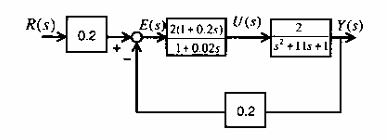
\includegraphics[width=0.5\linewidth]{figs/Q.42 image.png}
     \caption{figure}
     \label{fig:figs/Q.37 image.png}
 \end{figure}
      The steady state gain of the closed loop system, between output Y(s) and set point R(s), is 
  \hfill{(GATE 2010 CH)}\\

\begin{enumerate}
    \item 5/9
    \item 4/9
    \item 1/3
    \item 2/9
    
\end{enumerate}
\item 
   
   Consider the cascade control configuration shown in the figure below:\\

\begin{figure}[H]
    \centering
    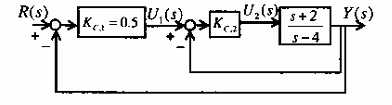
\includegraphics[width=0.5\linewidth]{figs/Q.43 image.png}
    \caption{figure}
    \label{fig:figs/Q.43 image.png}
\end{figure}
 
     The system is stable when Kc is
\hfill{(GATE 2010 CH)}\\
     \begin{enumerate}
         \item 3/4
         \item 1
         \item 5/4
         \item 3/2
         \end{enumerate}
\item 
  Consider the as shown below:
  
\begin{figure}[H]
    \centering
    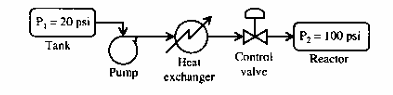
\includegraphics[width=0.5\linewidth]{figs/Q.44 image.png}
    \caption{figure}
    \label{fig:figs/Q.44 image.png}
\end{figure}
  
    A constant head pump transfers a liquid from a tank maintained at 20 psi to a reactor operating at 100 psi, through a heat exchanger and a control valve. At the design conditions, the liquid flow rate is 1000 litres/min, while the pressure drop across theheat exchanger is 40 psi, and that across the control valve is 20 psi. Assume that the pressure drop across the heat exchanger varies as the square of the flow rate. If the flow is reduced to 500 litres/min, then the pressure drop across the control valve is
    
\hfill{(GATE 2010 CH)}\\

    \begin{enumerate}
        \item 30 psi
        \item 50 psi
        \item 80 psi
        \item 150 psi
    \end{enumerate}
\item 
   A reactor needs to be lined with a corrosion resistant lining. One type of lining costs Rs. 5 lakhs, and is expected to last for 2 years. Another type of lining lasts for 3 years. If both choices have to be equally economical, with the effective interest rate being 18\%, compounded annually, the price one should pay for the second type of lining is
   \hfill{(GATE 2010 CH)}\\

   \begin{enumerate}
       \item Rs.6.1 lakhs
       \item Rs.6.5 lakhs
       \item Rs.6.9 lakhs
       \item Rs.7.6 lakhs
   \end{enumerate}
\item 
Match each of the following techniques of polymerisation in GROUP I, with the corresponding process characteristics in GROUP II.

 
      \begin{center}
\begin{tabular}{|c|c|c|}
    \hline
    Task & Task time (Seconds) & Immediate predecessor(s) \\
    \hline
    P & 20 & - \\ \hline
    Q & 25 & P \\  \hline
    R & 10 & Q \\ \hline
    S & 15 & Q \\ \hline 
    T & 25 & R, S \\    \hline
\end{tabular}
\end{center}
      
 \hfill{(GATE 2010 CH)}\\


\begin{enumerate}
    \item P-I, Q-II, R-III, S-IV
    \item P-II, Q-I, R-III, S-IV
    \item P-I, Q-II, R-IV, S-III
    \item P-III, Q-II, R-IV, S-I
\end{enumerate}
\item 
Match each of the polymers in GROUP I, with the raw material in GROUP II, from which they are made.
\begin{table}[h!]
\centering
\begin{tabular}{|c|c|c|c|}
\hline
\textbf{Pressure} & \textbf{Temperature} & \multicolumn{2}{c|}{\textbf{Specific enthalpy}} \\ \cline{3-4} 
\textbf{(kPa)} & \textbf{($^\circ$C)} & $h_f$ (kJ/kg) & $h_g$ (kJ/kg) \\ \hline
150.9 & $-20$ & 17.82 & 178.74 \\ \hline
500 & 15.6 & 50.64 & 195.01 \\ \hline
\end{tabular}
\end{table}
\begin{enumerate}
    \item P-I,Q-II,R-III,S-IV
    \item P-II,Q-I,R-III,S-IV
    \item P-I,Q-II,R-IV,S-III
    \item P-III,Q-II,R-IV,S-I
\end{enumerate}
\section{Common Data Questions}
\subsection{Common Data Questions 48 and 49:}

Hot oil at 150'C is used to preheat a cold fluid at 30'C in a  1 : 1 shell and tube heat exchanger. The exit temparature of the hot oil is 110'C. Heat capacities (product of mass rate and specific heat capacity ) of both the streams are equal. The heat duty is 2 kW.\\ 
\item 
  Under co-current flow conditions, the overall heat transfer resistance(l/UA) is
  \hfill{(GATE 2010 CH)}\\
  \begin{enumerate}
      \item 0.4'C/W
      \item 0.04'C/W
      \item 0.36'C/W
      \item 0.036'C/W
  \end{enumerate}
\item 
    Under counter-current flow conditions, the overall heattransfer resistance (l/UA) is
 
 \hfill{(GATE 2010 CH)}\\
 
  \begin{enumerate}
      \item 0.4'C/W
      \item 0.04'C/W
      \item 0.36'C/W
      \item 0.036'C/W
  \end{enumerate}

\subsection{Common Data Questions 50 and 51:}

A plant produces phenol. The variable cost in rupees per tonne of phenol is related to the plant capacity P(in tonnes/day) as 45,000 + 5P. The fixed charges are Rs. 100,000 per day. The selling price of phenol is Rs. 50,000 per tonne.\\
\item 
 The optimal plant capacity (in tonnes per day) for minimum cost per tonne of phenol, is
   
 \hfill{(GATE 2010 CH)}\\

\begin{enumerate}
    \item 101
    \item 141
    \item 283
    \item 422
\end{enumerate}
\item 
 The break-even capacity in tonnes per day, is
\hfill{(GATE 2010 C)}\\

\begin{enumerate}
    \item 50
    \item 40
    \item 30
    \item 20
    
\end{enumerate}

\section{Linked Answer Questions }
  \subsection{ Statements for Linked Answer Questions 52 and 53:} 

 Water is used to absorb ammonia from a gas mixture in a single separation stage contactor. The process is schematically represented in the figure below.

  \begin{figure}[H]
      \centering
      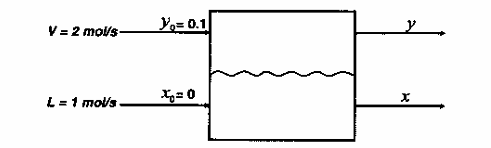
\includegraphics[width=1.0\linewidth]{figs/Q.52 image.png}
      \caption{figure}
      \label{fig:figs/Q.52 image.png}
  \end{figure}

  The molar gas and liquid flow rates, and the inlet molefractions are given in the figure. Both the liquid and the gas phases are well mixed, and the equilibrium relation between y and x is given by y* = x.
\item 
   If the stage is ideal, then the value of y is
   \hfill{(GATE 2010 CH)}\\
   
 \begin{enumerate}
     \item 1/15
     \item 1/10
     \item 1/4
     \item 1/3
 \end{enumerate}
\item 
  If the stage efficiency is 50\%, then the value of y is
  \hfill{(GATE 2010 CH)}\\

\begin{enumerate}
    \item 1/12
    \item 1/6
    \item 1/4
    \item 1/3
\end{enumerate}

\subsection{ Statements for Linked Answer Questions 54 and 55:} 

 A liquid phase reaction, A $\rightarrow $ B, is conducted isothermally in a CSTR having a residence time of 2 s. The rate law for the reaction is  

\begin{figure}[H]
    \centering
    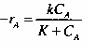
\includegraphics[width=0.25\linewidth]{figs/Q.54 image.png}
    \caption{figure}
    \label{fig:figs/Q.54 image.png}
\end{figure}
   
 where k=5 moles/litre/s.
 \item 
 The value of K, in moles/litre, is
\hfill{(GATE 2010 CH)}\\

\begin{enumerate}
    \item 11
    \item 9
    \item 5
    \item 2
    
\end{enumerate}
\item
 If the same reaction is conducted in a series of two CSTRs with residence time 1s and 0.2s, then the inlet concentration of A of 1 mole/litre, is
\hfill{(GATE 2010 CH)}\\

 \begin{enumerate}
     \item 2.64
     \item 2.00
     \item 1.64
     \item 0.54
     
 \end{enumerate}

\section{General Aptitude (GA) Questions}
\subsection{Q.56-Q.60 carry one mark each.}
\item 
 Choose the most appropriate word from the options given below to complete the following sentence:\\
 His rather casual remarks on politics \makebox[3cm]{\hrulefill} his lack of seriousness about the subject.
  
  \hfill{(GATE 2010 CH)}\\

  \begin{enumerate}
      \item masked
      \item belied
      \item betrayed
      \item suppressed
  \end{enumerate}
\item 
 Which of the following options is the closest in meaning to the word below:\\
     \textbf{Circuitous}
   
    \hfill{(GATE 2010 CH)}\\
 
 \begin{enumerate}
     \item cyclic
     \item indirect
     \item confusing
     \item crooked
 \end{enumerate}
\item 
 Choose the most appropriate word from the options given below to complete the following sentences:

  If we manage to \makebox[3cm]{\hrulefill} our natural resources, we would leave a better planet for our children.

\hfill{(GATE 2010 CH)}\\

\begin{enumerate}
    \item uphold
    \item restrain
    \item cherish
    \item conserve
\end{enumerate}
\item
 25 persons are in a room, 15 of them play hockey, 17 of them play football and 10 of them play both hockey and football. Then the number of persons playin neitherhockey nor football is:

 \hfill{(GATE 2010 CH)}\\

 \begin{enumerate}
     \item 2
     \item 17
     \item 13
     \item 3
     
 \end{enumerate}
\item
  The question below consists of a pair of related words followed by four pairs of words. Select the pair that best express the relation in the original pair.\\
 
  \hfill{(GATE 2010 CH)}\\
  
  \textbf{Unemployed : Worker}

\begin{enumerate}
    \item fallow : land
    \item unware : sleeper
    \item wit : jester
    \item renovated : house
\end{enumerate}

\subsection{Q.61-Q.65 carry two mark each.}
\item 
 If 137 + 276 = 435 how much is 731 + 672?

\hfill{(GATE 2010 CH)}\\

 \begin{enumerate}
     \item 534
     \item 1403
     \item 1623
     \item 1513
 \end{enumerate}
\item
 Hari (H), Gita (G), Irfan (I) and Saira (S) are siblings (i.e. brothers and sisters). All were born on 1$^{st}$ January. The age difference between any two successive siblings (that is born one after another) is less than 3 years. Given the following facts:\\
\begin{itemize}
    \item[i.] Hari's age + Gita's age $>$ Irfan's age + Saira's age.
    \item[ii.] The age difference between Gita and Saira is 1 year. However, Gita is not the oldest and Saira is not the youngest.
    \item[iii.] There are no twins.
\end{itemize}
In what order were they born (oldest first)?\\

\hfill{(GATE 2010 CH)}\\
\begin{enumerate}
    \item HSIG 
    \item SGHI
    \item JGSH
    \item HSGI
\end{enumerate}

\item 
 \textbf{Modern warfare has changed from large scale clashes of armies to suppression of civilian populations. Chemical agents that do their work silently appear to be suited to such warfare; and regretfully, there exist people in military establishments who think that chemical agents are useful tools for their cause.}

\noindent\textit{Which of the following statements best sums up the meaning of the above passage:}

\hfill{(GATE 2010 CH)}\\

\begin{enumerate}
    \item Modern warfare has resulted in civil strife.
    \item Chemical agents are useful in modern warfare.
    \item Use of chemical agents in warfare would be undesirable.
    \item People in military establishments like to use chemical agents in war.
\end{enumerate}
\item 
 5 skilled workers can build a wall in 20 days; 8 semi-skilled workers can build a wall in 25 days; 10 unskilled workers can build a wall in 30 days. If a team has 2 skilled, 6 semi-skilled and 5 unskilled workers, how long will it take to build the wall?\\

\hfill{(GATE 2010 CH)}\\

\begin{enumerate}
    \item 20 days
    \item 18 days
    \item 16 days
    \item 15 days
\end{enumerate}
\item 
Given digits 2, 2, 3, 3, 3, 4, 4, 4, 4 how many distinct 4 digit numbers greater than 3000 can be formed ?

\hfill{(GATE 2010 CH)}\\

\begin{enumerate}
    \item 50
    \item 51
    \item 52
    \item 54
\end{enumerate}
 \end{enumerate}
\end{document}








